\documentclass[12pt]{article}%
% Used for centring the title
\usepackage{titlesec}
\titleformat{\section}[block]{\Large\bfseries\filcenter}{}{1em}{}

% Packages
\usepackage{amsfonts}
\usepackage{fancyhdr}
\usepackage{comment}
\usepackage[a4paper, top=2.5cm, bottom=2.5cm, left=2.2cm, right=2.2cm]%
{geometry}
\usepackage{times}
\usepackage{amsthm}
\usepackage{amsmath}
\usepackage{changepage}
\usepackage{amssymb}
\usepackage{graphicx}%
\usepackage{xcolor}
\usepackage{breqn}

% Theorem Formats
\setcounter{MaxMatrixCols}{30}
\newtheorem{theorem}{Theorem}
\newtheorem{acknowledgement}[theorem]{Acknowledgement}
\newtheorem{algorithm}[theorem]{Algorithm}
\newtheorem{axiom}{Axiom}
\newtheorem{case}[theorem]{Case}
\newtheorem{claim}[theorem]{Claim}
\newtheorem{conclusion}[theorem]{Conclusion}
\newtheorem{conjecture}[theorem]{Conjecture}
\newtheorem{corollary}[theorem]{Corollary}
\newtheorem{criterion}[theorem]{Criterion}
\newtheorem{definition}[theorem]{Definition}
\newtheorem{example}[theorem]{Example}
\newtheorem{exercise}[theorem]{Exercise}
\newtheorem*{claim*}{Claim}
\newtheorem{lemma}[theorem]{Lemma}
\newtheorem{notation}[theorem]{Notation}
\newtheorem{problem}[theorem]{Problem}
\newtheorem{proposition}[theorem]{Proposition}
\newtheorem{remark}[theorem]{Remark}
\newtheorem{solution}[theorem]{Solution}
\newtheorem{summary}[theorem]{Summary}

% new commands for readability
\newcommand{\C}{\mathbb{C}}
\newcommand{\F}{\mathbb{F}}
\newcommand{\N}{\mathbb{N}}
\newcommand{\Q}{\mathbb{Q}}
\newcommand{\R}{\mathbb{R}}
\newcommand{\Z}{\mathbb{Z}}
\newcommand{\Mod}[1]{\ (\mathrm{mod}\ #1)}
\newcommand{\rpm}{\raisebox{.2ex}{$\scriptstyle\pm$}}

\begin{document}

% Title
\title{Assignment 2}
\author{Robert Lech}
\date{\today}
\maketitle
\section*{Chapter 3}

\subsection*{Question 13}

\begin{claim*}
Show that $A*B$ is a free group if and only if $A$ and $B$ are free.
\end{claim*}

\begin{proof}
$(\Rightarrow)$ Assume $A*B$ is a free group. We'd like to show that $A$ and $B$ are free. Firstly, we
note that $A$ and $B$ are definitely subgroups of $A*B$. This can be seen in Corollary 3.27 that states
that groups $A$ and $B$ inject into $A*B$. Therefore, we can use Corollary 3.23 (Nielsen-Schreier) to say
that the subgroups $A$ and $B$ are themselves free.

$(\Leftarrow)$ Assume $A$ and $B$ are free groups. Then there exist bases $S_A$ and $S_B$ such that
$A=<S_A>$ and $B=<S_B>$ and no non-trivial, freely reduced word represents the identity $1_A$ and $1_B$,
respectively. We want to show $A*B$ is free. That is, we want to show there exists a basis $S_{A*B}$ such
that $<S_{A*B}>=A*B$ and no non-trivial freely reduced word represents the identity $1_{A*B}$,
respectively.

Therefore, we can let $S_{A*B}=S_A \cup S_B$. We also note that, without loss of generality, every word in
$A*B$ is of the form $w=a_{1}b_{1}a_{2}b_{2}\ldots a_{n}b_{n}$ for some $a_i\in A$, $a_i \neq 1_A, \forall
i=2,3,\ldots n$ and $b_i\in B$, $b_j \neq 1_B, \forall i=1,2,\ldots n-1$. Moreover, this word doesn't
freely reduce. That is, for all $i\in {1, 2, \ldots n}$, $b_{i-1} \neq a_i \neq b_i$ and $b_{i-1} \neq
a_i^{-1} \neq b_i$ (as they were from different groups)

Therefore, this word cannot freely reduce to $1_{A*B}$. Therefore, $A*B$ must be free.
\end{proof}

\subsection*{Question 14}

Let $\F_2$ be a free group with basis $\{x,y\}$, and let $K$
 be the kernel of the homomorphism $\phi:\F_2\rightarrow \Z_3$ induced by $\phi(x)=\phi(y)=1$.

% Taken from: https://www.sharelatex.com/learn/Lists
\renewcommand{\labelenumi}{\alph{enumi}}
\begin{enumerate}
  \item Find the fundamental domain for the action of $K$ on the Cayley graph of $\F_2$.
\end{enumerate}

\subsubsection*{Before we begin}

We should note that since $\phi$ is a group homomorphism, we can determine the values of $\phi(x^3)$ and
$\phi(x^{-1})$. We see that $\phi(x^3)=\phi(x*x*x)=\phi(x)+\phi(x)+\phi(x)=1+1+1=0$. On the other hand,
$0=\phi(1)=\phi(x*x^{-1})=\phi(x)+\phi(x^{-1})$. Therefore:

\begin{align*}
\phi(x)+\phi(x^{-1})=0
&\implies 1+\phi(x^{-1})=0\\
&\implies 3+\phi(x^{-1})=2\\
&\implies \phi(x^{-1})=2
\end{align*}

Therefore, $\phi(x^3)=0$ and $\phi(x^{-1})=2$.  Similarly  $\phi(y^3)=0$ and $\phi(y^{-1})=2$.

\subsubsection*{How does $K$ look}

Firstly, suppose we have the set $K'$ such that:
\begin{align*}
K'
&=\{e\} \\
&\cup\{xy^{-1}, x^{-1}y, (xy^{-1})^{-1}, (x^{-1}y)^{-1}\} \\
&\cup\{xxx,xxy,xyx,xyy,yxx,yxy,yyx,yyy, \\
&(xxx)^{-1},(xxy)^{-1},(xyx)^{-1},(xyy)^{-1},(yxx)^{-1},(yxy)^{-1},(yyx)^{-1},(yyy)^{-1}\} \\
&\cup \ldots
\end{align*}

Therefore, as proven below, we can think of $K'$ as the words with exponents adding up to $0 \Mod{3}$.
More formally, $K'=\{a_{1}^{\varepsilon_1}a_{2}^{\varepsilon_2}\ldots a_{n}^{\varepsilon_n} | a_i\in \F_2,
\varepsilon_i\in \{-1, 1\}, \sum_{i=1}^{n} \varepsilon_i \equiv 0 \Mod{3}\}$.

\begin{claim}
$K'=K$
\end{claim}

\begin{proof}
We first begin by showing $K' \subseteq K$. That is, suppose
$w=a_{1}^{\varepsilon_1}a_{2}^{\varepsilon_2}\ldots a_{n}^{\varepsilon_n}$ where $a_i\in \F_2,
\varepsilon_i\in \{-1, 1\}, \sum_{i=1}^{n} \varepsilon_i \equiv 0 \Mod{3}$. Then:

\begin{align*}
\phi(w)
&=\phi(a_{1}^{\varepsilon_1}a_{2}^{\varepsilon_2}\ldots a_{n}^{\varepsilon_n}) \\
&=\phi(a_{1}^{\varepsilon_1})+\phi(a_{2}^{\varepsilon_2})+\cdots +\phi(a_{n}^{\varepsilon_n}) \\
&=\sum_{\varepsilon_i=1}  \phi(a_{i}^{\varepsilon_i})+\sum_{\varepsilon_i=-1}  \phi(a_{i}^{\varepsilon_i}) \\
&=\sum_{\varepsilon_i=1}  \phi(a_{i})+\sum_{\varepsilon_i=-1}  \phi(a_{i}^{-1}) \\
&=\sum_{\varepsilon_i=1}  1+\sum_{\varepsilon_i=-1}  2 \\
&\equiv 0 \Mod{3}
\end{align*}

Therefore, $w\in \ker(\phi)$ and so $K' \subseteq K$. Not we show that $K \subseteq K'$. That is, assume
$\phi(w)=0$, for some $w=a_{1}^{\varepsilon_1}a_{2}^{\varepsilon_2}\ldots a_{n}^{\varepsilon_n}$ where
$a_i\in \F_2, \varepsilon_i\in \{-1, 1\}$. We need to show that $\varepsilon_i \equiv 0 \Mod{3}$. However:

\begin{align*}
\phi(w)
&=\phi(a_{1}^{\varepsilon_1}a_{2}^{\varepsilon_2}\ldots a_{n}^{\varepsilon_n}) \\
&=\phi(a_{1}^{\varepsilon_1})+\phi(a_{2}^{\varepsilon_2})+\cdots +\phi(a_{n}^{\varepsilon_n}) 
\end{align*}

However, we know that $\phi(x)=\phi(y)$ and $\phi(x^{-1})=\phi(y^{-1})$. So without loss of generality:

\begin{align*}
\phi(w)
&=\phi(a_{1}^{\varepsilon_1})+\phi(a_{2}^{\varepsilon_2})+\cdots +\phi(a_{n}^{\varepsilon_n}) \\
&=\phi(x^{\varepsilon_1})+\phi(x^{\varepsilon_2})+\cdots +\phi(x^{\varepsilon_n}) \\
&=\phi(x^{\varepsilon_1}x^{\varepsilon_2}\ldots x^{\varepsilon_n}) \\
&=\phi(x^{\varepsilon_1+\varepsilon_2+\cdots +\varepsilon_n}) \\
&=\phi(x)^{\varepsilon_1+\varepsilon_2+\cdots +\varepsilon_n}
\end{align*}

However, $\phi(w)=0$. Therefore, $\phi(x)^{\varepsilon_1+\varepsilon_2+\cdots +\varepsilon_n}=0$. But
since $\phi(x)=1$ we have that $1+1+\cdots+1\equiv 0\Mod3$ (where we have
$\varepsilon_1+\varepsilon_2+\cdots +\varepsilon_n$ ones). However, this implies 
$\varepsilon_1+\varepsilon_2+\cdots +\varepsilon_n \equiv 0 \Mod{3}$. Therefore, $w\in K'$ and so 
$K\subseteq K'$.

In conclusion, $K=K'$.

\end{proof}

\textbf{The Cayley Graph for $\F_2$ and the Fundamental Domain for $K$}

As seen in the book in Figure 3.1 and as claimed in Corollary 3.4 on page on page 56, the free group
$\F_2$ can be viewed as a group of symmetries of $\mathcal{T}_4$. The fundamental domain, $\mathcal{F}$,
that I'm choosing for $K$, will initially consist of vertex $e$. To know what other vertices get added to
$\mathcal{F}$, we can note that for every word $k\in K$ and for every $w\not\in K$, it can be shown that
$wk\not\in K$. That is, $wk$ is not a word with exponents adding up to $0\Mod{k}$. Therefore vertices $x$
and $x^2$, along with the edges between ($e$ and $x$) and ($x$ and $x^2$) can be added to $\mathcal{F}$.
Lastly, adding the half-edges connected to the three vertices gives us $\mathcal{F}$. This can all be seen
in Figure~\ref{fig:fun_domain_of_K} below.

\begin{figure}[ht]
    \centering
    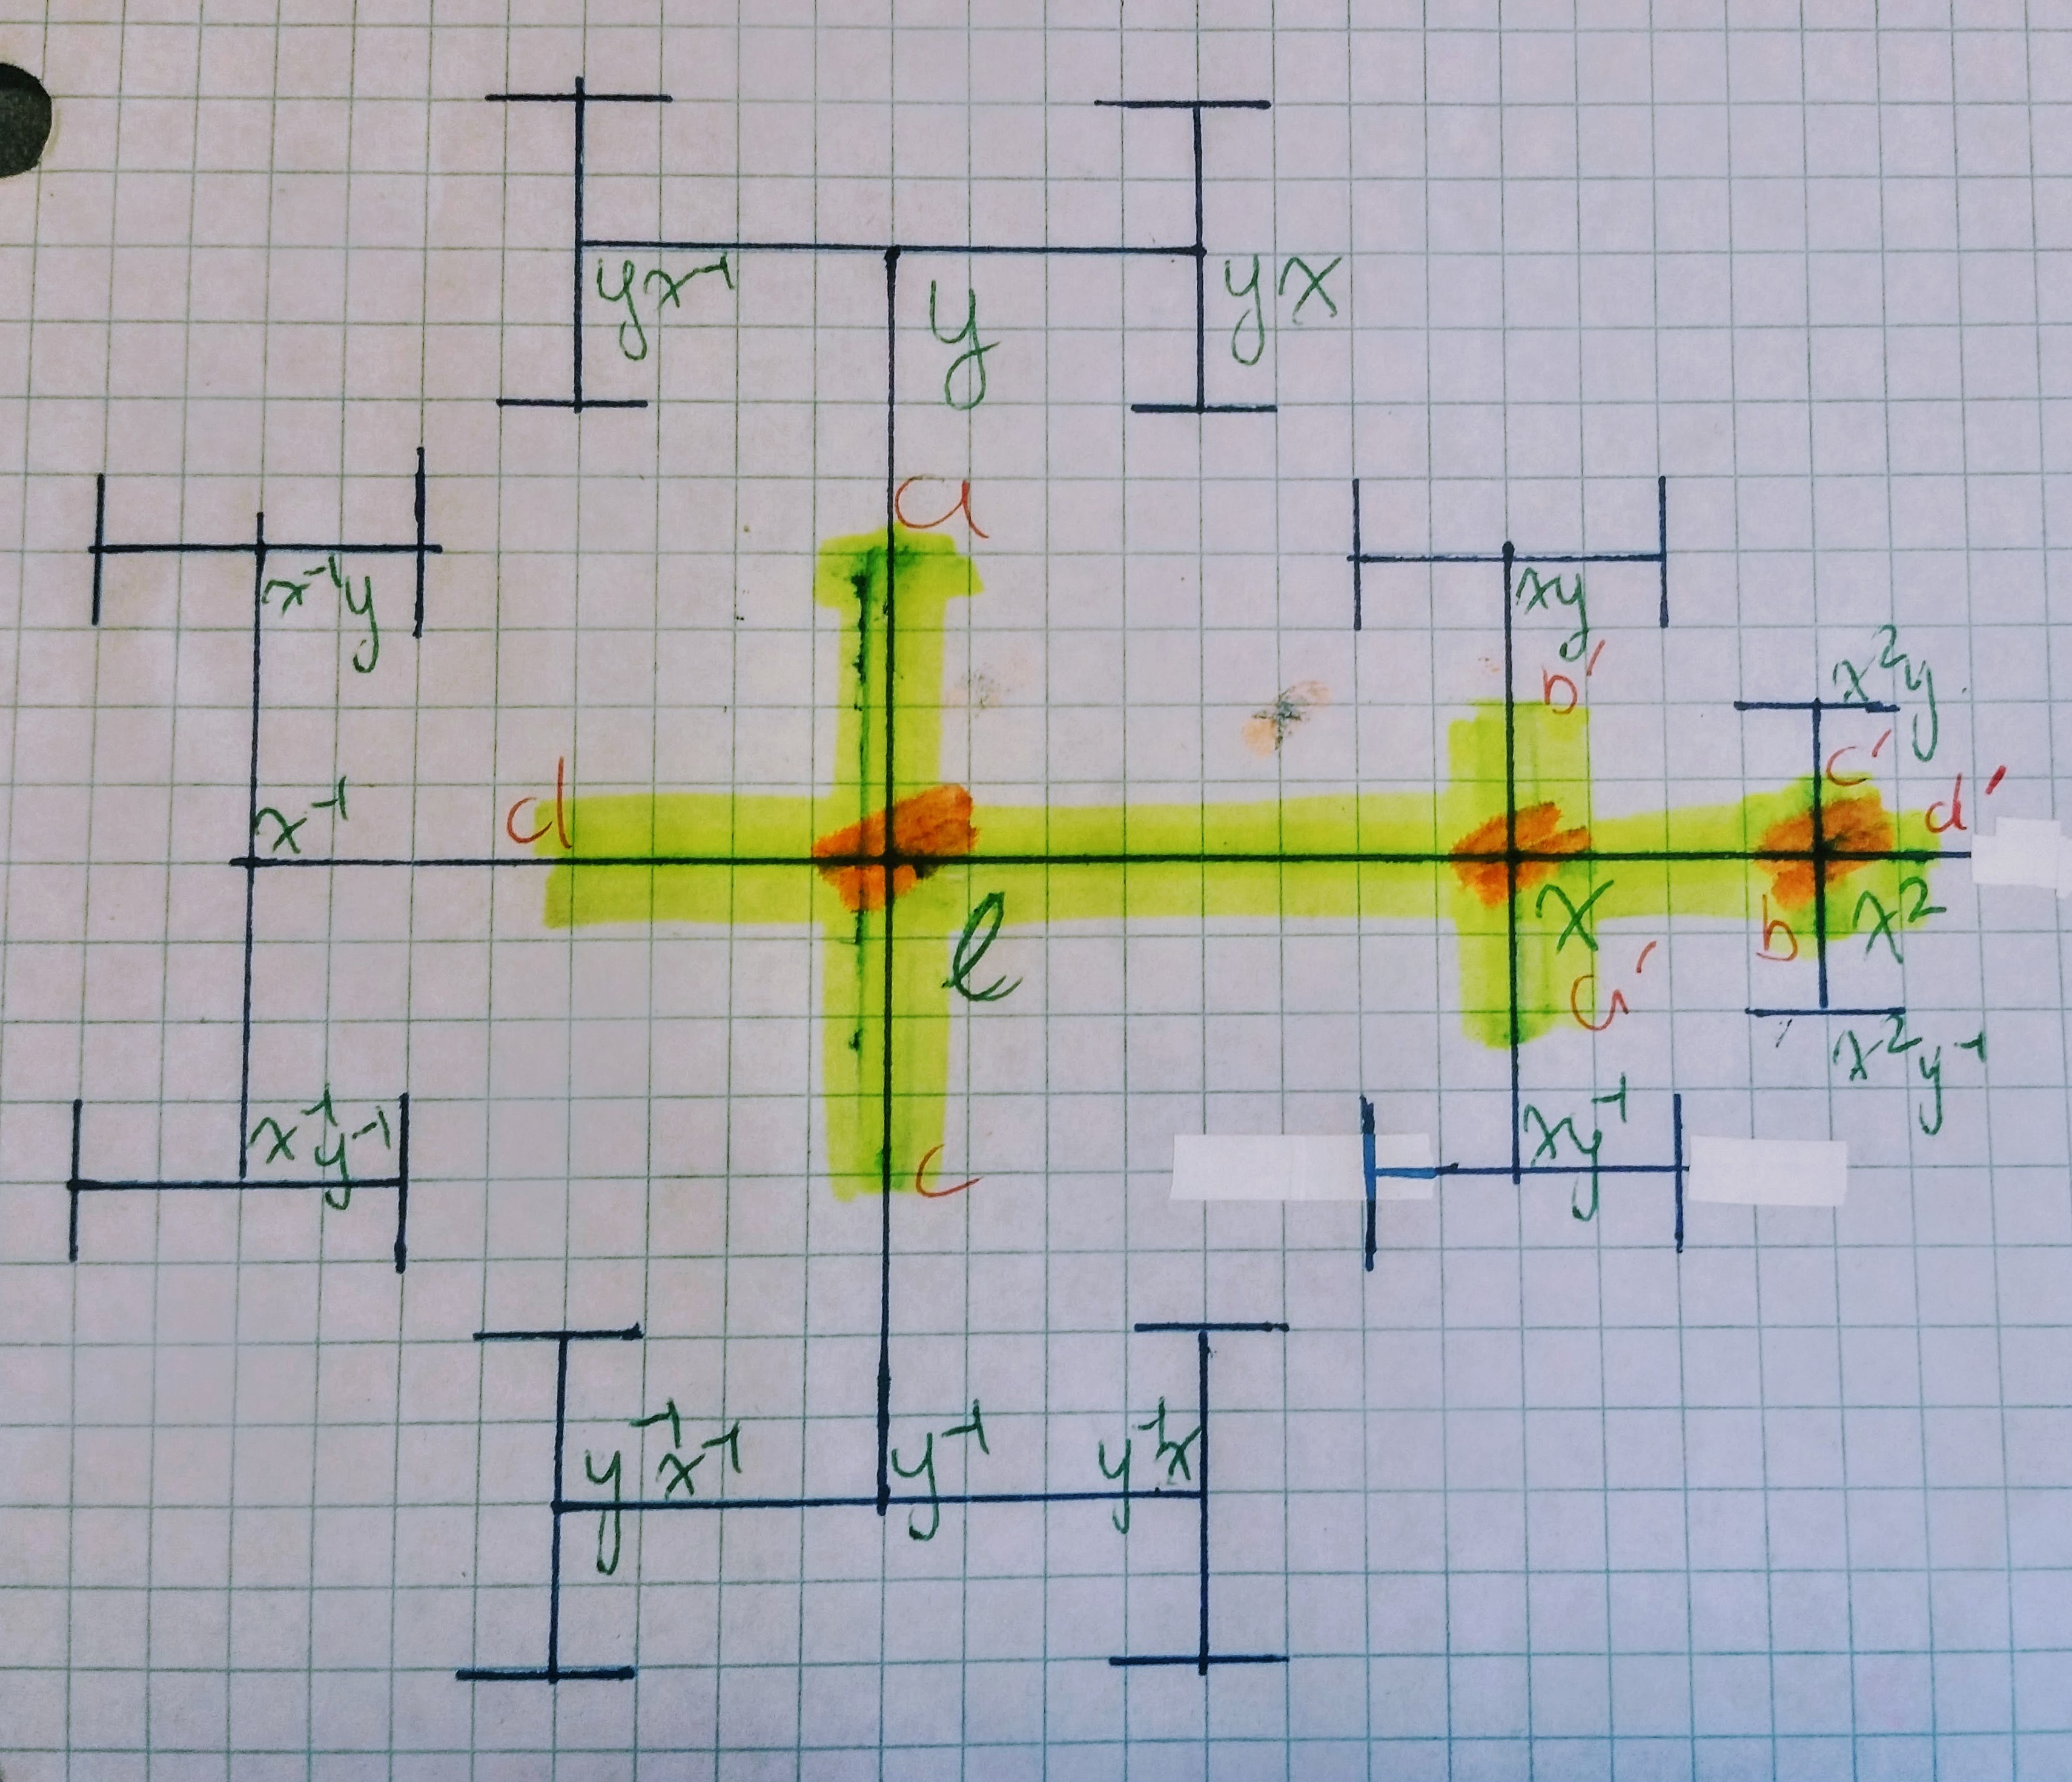
\includegraphics[width=0.9\textwidth]{images/fundamental_domain_for_K.jpg}
    \caption{The Cayley graph for $\F_2$ and the fundamental domain, $\mathcal{F}$, for $K$. Also listed are labels for endpoints of half-edges attached to vertices in $\mathcal{F}$.}
    \label{fig:fun_domain_of_K}
\end{figure}

\begin{enumerate}
  \setcounter{enumi}{1}
  \item Find a basis $S$ for the kernel $K$.
\end{enumerate}

Using Figure~\ref{fig:fun_domain_of_K} as a visual aid, we see there are eight half-edges in
$\mathcal{F}$. This implies there should be four elements in our basis $S$ such that $S^{\rpm}=\left\{g\in
K | g\mathcal{F} \cap \mathcal{F} \neq \emptyset \right\}$. These should be the elements that map ends of
half-edges in $\mathcal{F}$ to ends of half-edges $\mathcal{F}$.  Good ones to start with are the words in
the kernel that have `minimal' length. Apart from the identity, these are the words listed at the
beginning of this question. Start by adding $xy^{-1}$ (which can map point $a$ to $a'$) and $x^{-1}y$
(which can map point $b$ to $b'$) to $S$ as they are not inverses of each other. We proceed by adding
$xxx$ (which can map point $c$ to $c'$) to $S$. We also note these three words generate $xyy$, $yyx$,
and $yyy$. We finally add $xyx$ (which can map point $d$ to $d'$) to $S$. We also note that $xy^{-1},
x^{-1}y$, and $xyx$ generate the remaining words $xxy$, $yxx$, and $yxy$. 

At this point, all words of length 2 and 3 can be generated. Therefore, the basis for $\mathcal{F}$ is
$S=\left\{xy^{-1}, x^{-1}y, xxx, xyx\right\}$.

\subsection*{Question 18}

\begin{claim*}
Let $A$ and $B$ be non-trivial groups. Prove that the centre of $A*B$ is trivial.
\end{claim*}

\begin{proof}
Let $A$ and $B$ be non-trivial groups. Denote the centre of $G$ as
$Z(A*B)=\{ w \in A*B | wx=xw, \forall x \in A*B \}$. Clearly the identity is in $Z(A*B)$ since the
identity must commute with every element in a group. However, to prove that no other elements in $A*B$ are
in $Z(A*B)$, we'll do a proof by contradiction. That is, we'll suppose there exists a $w\in Z(A*B)$ such
that $w \neq 1_{A*B}$. Then this $w$ commutes with every word $x \in A*B$. We'll show this is impossible
by finding a word, in every case, that cannot possibly commute with $w$.

\textbf{Case 1}: Suppose $w=a_{1}b_{1}a_{2}b_{2}\ldots a_{n}b_{n}$, where
$a_1,a_2,\ldots ,a_n, b_1,b_2,\ldots b_n$ are not the identity and $n\geq 1$. Then let $x=a_1$ and look
at the word $wxw^{-1}x^{-1}$. We see that:

\begin{align*}
  wxw^{-1}x^{-1} &= (a_{1}b_{1}a_{2}b_{2}\ldots a_{n}b_{n}) (a_{1}) (b_{n}^{-1}a_{n}^{-1}\ldots b_{2}^{-1}a_{2}^{-1}b_{1}^{-1}a_{1}^{-1}) (a_{1}^{-1}) \\
  &\neq 1
\end{align*}

as it doesn't freely reduce.

\textbf{Case 2}: Suppose $w=b_{1}a_{1}b_{2}a_{2}\ldots b_{n}a_{n}$, where
$a_1,a_2,\ldots ,a_n, b_1,b_2,\ldots b_n$ are not the identity and $n\geq 1$. Then let $x=b_1$ and refer
to \textbf{Case 1} for the proof structure. 

\textbf{Case 3.a}:
Suppose $w=a$, where $a$ is not the identity in $A$. Then let $x=b$ for some $b\in B$ and look at the word
$wxw^{-1}x^{-1}$. We see that $wxw^{-1}x^{-1}=aba^{-1}b^{-1}$ which does not reduce freely.

\textbf{Case 3.b}: 
Suppose $w=a_{1}b_{1}a_{2}b_{2}\ldots a_{n}$, for $n\geq 2$ and where $a_1,a_2,\ldots ,a_n, b_1,b_2,\ldots b_{n-1}$ are not the identity. Then let $x=b_{n-1}$ and look at the word $wxw^{-1}x^{-1}$. We see that:

\begin{align*}
  wxw^{-1}x^{-1} &= (a_{1}b_{1}a_{2}b_{2}\ldots a_{n}) (b_{n-1}) (a_{n}^{-1}\ldots b_{2}^{-1}a_{2}^{-1}b_{1}^{-1}a_{1}^{-1}) (b_{n-1}^{-1}) \\
  &\neq 1
\end{align*}

as it doesn't freely reduce.

\textbf{Case 4.a}:
Suppose $w=b$, where $b$ is not the identity in $B$. Then let $x=a$ for some $a\in B$ and look at the word
$wxw^{-1}x^{-1}$. We see that $wxw^{-1}x^{-1}=bab^{-1}a^{-1}$ which does not reduce freely.

\textbf{Case 4.b}: Suppose $w=b_{1}a_{1}b_{2}a_{2}\ldots b_{n}$, for $n\geq 2$ and where
$a_1,a_2,\ldots ,a_{n-1}, b_1,b_2,\ldots b_n$ are not the identity. Then let $x=a_{n-1}$ and refer to
\textbf{Case 3} for the proof structure. 

Since these 4 cases represent every non-trivial, reduced word in $A*B$, we see that that $Z(A*B)$ must
be trivial.
\end{proof}

\section*{Chapter 4}

\subsection*{Question 7}

Prove that the smallest normal subgroup of $BS(1, 2)$ that contains $b$ is isomorphic to the dyadic
rationals.

\textbf{Step 1: Find the smallest normal subgroup $BS(1,2)$ containing $b$.}

We'll first note what facts we'll need for this problem. Firstly, we note that $BS(1,2)=<a,b|aba^1=b^2>$,
where $a(x)=2x$ and $b(x)=x+1$.  From Proposition 4.1 on page 102 in the book, we know that:

\begin{equation}
BS(1,2)=\left\{g_{k,m,n}(x) | g_{k,m,n}(x)=\frac{2^{n+k}x+m}{2^k}, \forall k, m, n \in \Z \right\}
\end{equation}

Now, the question is asking us for the smallest normal subgroup of $BS(1,2)$ that contains $b$. There is a
fact that the conjugate/normal closure of a generating set $S$ is precisely this. The normal closure is
defined as $S^G=\left\{g^{-1}sg|\forall g\in G, s\in S\right\}$. Since $S=<b>$, this simplifies to
$S^G=\left\{g^{-1}b^{i}g|\forall g\in G, \forall i \in \Z \right\}$. Therefore, for some $k, m, n, i$, we
can compute $g_{k,m,n}^{-1}(b^{i}(g_{k,m,n}(x)))$. We note that:

\begin{itemize}
\item $g_{k,m,n}(x)=\frac{2^{n+k}x+m}{2^k}$ 
\item $g_{k,m,n}^{-1}(x)=\frac{2^{n+k}x-m}{2^k}$ 
\item $b^{i}(x)=x+i$ % chktex 17
\end{itemize}
% chktex 17
Below, we see it simplifies to:

\begin{align*}
g_{k,m,n}^{-1}(b^{i}(g_{k,m,n}(x)))
&= g_{k,m,n}^{-1}\left(b^{i}\left(\frac{2^{n+k}x+m}{2^k}\right)\right) \\
&= g_{k,m,n}^{-1}\left(\frac{2^{n+k}x+m}{2^k}+i\right) \\
&= g_{k,m,n}^{-1}\left(\frac{2^{n+k}x+m+i2^k}{2^k}\right) \\
&= \frac{2^k\left(\frac{2^{n+k}x+m+i2^k}{2^k}\right)-m}{2^{n+k}} \\
&= \frac{2^{n+k}x+m+i2^k-m}{2^{n+k}} \\
&= \frac{2^{n+k}x+i2^k}{2^{n+k}} \\
&= x+\frac{i}{2^{n}}
\end{align*}

Therefore, $S^G=\left\{f_{i,n}(x)|f_{i,n}(x)=x+\frac{i}{2^{n}}, \forall n\in \Z\right\}$.\\

\textbf{Step 2: Show $S^G\simeq$  the group $\left(\Z\left[\frac{1}{2}\right],+\right)$}

To show the two that $S^G$ under function composition is group isomorphic to
$\left(\Z\left[\frac{1}{2}\right],+\right)$, we first need to show that $S^G$ under function composition
is even a group. \\

\textbf{Step 2.a: Show $S^G$ is a group under function composition.}

Therefore, to do this we need to show that: \\

\textbf{Step 2.a.i: Show $S^G$ is closed under composition.}

Let $f_{i,n}(x), f_{j,m}(x)$ be $\in S^G$. Then: 
\begin{align*}
f_{i,n}(f_{j,m}(x))
&=f_{i,n}(x+\frac{j}{2^{m}}) \\
&=x+\frac{i}{2^{m}}+\frac{j}{2^{n}} \\
&=x+\frac{i2^{n}+j2^{m}}{2^{m}2^{n}} \\
&=x+\frac{i2^{n}+j2^{m}}{2^{mn}}
\end{align*}
Reducing $\frac{i2^{n}+j2^{m}}{2^{mn}}$ gives us a distinct element in $S^G$.

\textbf{Step 2.a.ii: Show $S^G$ is associative under composition.}

Let $f_{i_1,n_1}(x), f_{i_2,n_2}(x), f_{i_3,n_3}(x)$ be $\in S^G$. Then we need to show that
$(f_{i_1,n_1}\circ f_{i_2,n_2}) \circ f_{i_3,n_3}=f_{i_1,n_1}\circ (f_{i_2,n_2} \circ f_{i_3,n_3})$.
Start with the left hand side.
$(f_{i_1,n_1}\circ f_{i_2,n_2}) \circ f_{i_3,n_3} = (x+\frac{i_2}{2^{n_2}}+\frac{i_1}{2^{n_1}}) \circ (x+\frac{i_3}{2^{n_3}}) = x+\frac{i_3}{2^{n_3}}+\frac{i_2}{2^{n_2}}+\frac{i_1}{2^{n_1}}$. On the other
hand, $f_{i_1,n_1}\circ (f_{i_2,n_2} \circ f_{i_3,n_3})=(x+\frac{i_1}{2^{n_1}})\circ (x+\frac{i_3}{2^{n_3}}+\frac{i_2}{2^{n_2}})=x+\frac{i_3}{2^{n_3}}+\frac{i_2}{2^{n_2}}+\frac{i_1}{2^{n_1}}$
. Since the two are equal, we see associativity holds. \\

\textbf{Step 2.a.iii: Show $S^G$ contains the identity map under composition.}

Let $f_{0,n}(x)=x+\frac{0}{2^n}=x$ be $\in S^G$.  Then it's clear that this is the identity composition. \\

\textbf{Step 2.a.iv: Show $S^G$ contains inverses for every element.}

Let $f_{i,n}(x)=x+\frac{i}{2^n}$ be $\in S^G$.  Then $f_{-i,n}(x)=x+\frac{-i}{2^n}$. Then it's clear that
$f_{i,n}(f_{-i,n}(x))=x$ and so they are inverses. \\

\textbf{Step 2.b: Find our mapping $\phi$}

First denote $\Z\left[\frac{1}{2}\right]=\{ \frac{i}{2^n} | i \in \Z, n \in \N \}$. Then we define our
mapping $\phi:S^G \rightarrow \Z\left[\frac{1}{2}\right]$to be $\phi(f_{i,n}(x))=\frac{i}{2^n}$. \\

\textbf{Step 2.c: Show $\phi$ is a bijection}

To show that the function is onto, note that for every reduced fraction
$\frac{i}{2^n} \in \Z[\frac{1}{2}]$, there exists a function (specifically $f_{i,n}(x)$) such that
$\phi(f_{i,n}(x))=\frac{i}{2^n}$. \\

To see that the mapping is one-to-one we suppose some reduced fractions
$\frac{i_{1}}{2^{n_1}}, \frac{i_{2}}{2^{n_2}} \in \Z[\frac{1}{2}]$ are such that
$\frac{i_{1}}{2^{n_1}} = \frac{i_{2}}{2^{n_2}}$. Adding $x$ to both sides gives us 
$x+\frac{i_{1}}{2^{n_{1}}}=x+\frac{i_{2}}{2^{n_{2}}}\Leftrightarrow f_{i_{1},n_{1}}(x)=f_{i_{2},n_{2}}(x)$. \\

Therefore, $\phi$ is a bijection. \\

\textbf{Step 2.d: Show $\phi$ is a homomorphism}

To show this is a group homomorphism, we note that if we take two functions
$f_{i_{1},n_{1}}, f_{i_{2},n_{2}} \in S^G$, then we see that:

\begin{align*}
\phi\left(f_{i_{2},n_{2}} \circ f_{i_{1},n_{1}}\right)
&=\phi \left(f_{i_{2},n_{2}}\left(x+\frac{i_{1}}{2^{n_1}}\right)\right) \\
&=\phi\left(x+\frac{i_{2}}{2^{n_2}}+\frac{i_{1}}{2^{n_1}}\right) \\
&=\frac{i_{2}}{2^{n_2}}+\frac{i_{1}}{2^{n_1}}
\end{align*}
Performing the mapping first, we see that:

\begin{align*}
\phi\left(f_{i_{2},n_{2}}(x)\right)+\phi\left(f_{i_{1},n_{1}}(x)\right)
&=\phi \left(x+\frac{i_{2}}{2^{n_2}}\right)+\phi \left(x+\frac{i_{1}}{2^{n_1}}\right) \\
&=\left(\frac{i_{2}}{2^{n_2}}\right) + \left(\frac{i_{1}}{2^{n_1}}\right) \\
&=\frac{i_{2}}{2^{n_2}}+\frac{i_{1}}{2^{n_1}}
\end{align*}

Since $\phi\left(f_{i_{2},n_{2}}(x)\right)\phi\left(f_{i_{1},n_{1}}(x)\right)=\phi\left(f_{i_{2},n_{2}} \circ f_{i_{1},n_{1}}\right)$,
we see that $\phi$ is a group homomorphism, and so $\phi$ is a group isomorphism as well. \\

This shows that $S^G\simeq \Z\left[\frac{1}{2}\right]$.

\end{document}
